	\begin{figure}[!h]
		\centering
 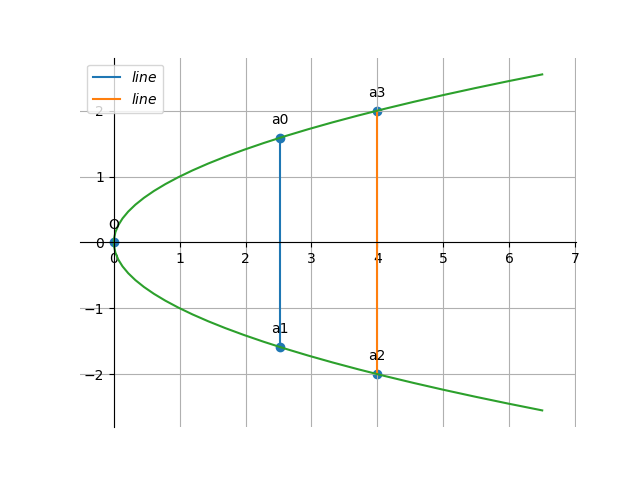
\includegraphics[width=\columnwidth]{chapters/12/8/1/8/figs/conics1.png}
		\caption{}
		\label{fig:12/8/1/8}
  	\end{figure}
The given conic parameters are
\begin{align}
 \vec{V} = \myvec{0 & 0\\0 & 1},
	\vec{u} = -\frac{1}{2}\vec{e}_1
 f = 0
\end{align}
The parameters of the lines are
\begin{align}
\vec{q}_2=\myvec{a\\0},
\vec{m}_2=\vec{e}_2
\end{align}
Substituting the above values in 
\eqref{eq:tangent_roots},
\begin{align}
\mu_i=a,-a
\end{align}
yielding  the points of  intersection as
\begin{align}
\vec{a_0}=\myvec{a\\a},
\vec{a_1}=\myvec{a\\-a}
\end{align}
Similarly, for the line $x-4=0$, 
\begin{align}
\vec{q_1}=\myvec{4\\0},
\vec{m_1}=\vec{e}_2
\end{align}
yielding
\begin{align}
\mu_i=2,-2
\end{align}
and
\begin{align}
\vec{a}_3=\myvec{4\\2},
\vec{a}_2=\myvec{4\\-2}.
\end{align}
Area between parabola and the line $x=4$ is divided equally by the line $x=a$.  Thus, 
		from \figref{fig:12/8/1/8},
\begin{align}
	A_1&=\int_{0}^{a} \ \sqrt{x} \,dx
	\\
	A_2&=\int_{a}^{4} \ \sqrt{x} \,dx
	\\
	\text{ and }
	A_1&=A_2 \\
\implies 
	a&=4^\frac{2}{3}
\end{align}

\iffalse
\section*{\large Construction}

{
\setlength\extrarowheight{5pt}
\begin{tabular}{|l|c|}
    \hline 
    \textbf{Points} & \textbf{intersection points} \\ \hline
   a0 & $\myvec{
   a\\
   a
   } $ \\\hline
   a1 & $\myvec{
   a\\
   -a
   } $ \\\hline
    
   a3 & $\myvec{
   4\\
   2
   } $ \\\hline
   a2 & $\myvec{
   4\\
   -2
   } $ \\\hline
      
      \end{tabular}
}

\end{document}
\fi
